% ************************* Preámbulo ********************************

% *************** Document Class ***************
% Para más información sobre las clases:
% https://en.wikibooks.org/wiki/LaTeX/Document_Structure#Document_classes
% En la tabla "Document classes"
% https://ctan.org/topic/class
% \documentclass[10pt, a4paper]{book}
\documentclass[12pt, oneside, a4paper, openright]{book} % \documentclass[options]{class}
% Si usas twoside en vez de oneside, LaTeX te pondrá hojas blancas adicionales

% Para más información sobre las opciones:
% https://en.wikibooks.org/wiki/LaTeX/Document_Structure#Document_classes
% En la tabla "Document Class Options"

% Posibles opciones:
% 10pt, 11pt, 12pt : El tamaño de la fuente por defecto
% a4paper, letterpaper,... : El tamaño del papel del documento
% twocolumn
% landscape
% titlepage, notitlepage
% openright, openany
% draft
% fleqn
% leqno

%------------ Paquetes, macros y metadata ------------%
% ************************ Thesis Information & Meta-data **********************

%------------Información básica------------%
\newcommand{\egilea}{Baldwin David Rodr\'{i}guez Ponce} % The full name of the author
\newcommand{\zuzendariak}{Mar\'{i}a Begoña Losada Pereda}

\newcommand{\upvehu}{Universidad de Granada} % University
\newcommand{\informatikafakultatea}{Escuela Técnica Superior de Ingenierías Informática y Telecomunicaciones}
\newcommand{\gradua}{Grado en Ingeniería Informática}  % Full title of the Degree
\newcommand{\espezialitatea}{Computación y Sistemas Inteligentes}

\newcommand{\izenburua}{Placeholder name for the game} % The title of the thesis
% \newcommand{\izenburua}{Simpy: Un lenguaje de modelado de sistemas de simulación dinámicos discretos} % The title of the thesis
\newcommand{\gapizenburua}{Game Design Document} % Subtitle
% \newcommand{\gapizenburua}{Proyecto de Fin de Grado}

\newcommand{\crest}{
\includegraphics[width=0.35\textwidth]{1-Portada/UGR_LOGO.png}} % University Crest (logo)
\newcommand{\data}{\today} % Submission date
\newcommand{\urtea}{2022}

\newcommand{\egileatestua}{Autor}
\newcommand{\zuzendariaktestua}{Directora}

\newcommand{\abstract}{Resumen}

% \message{LaTeX Warning: \noexpand Aviso! Mejor si cambias los textos 'Autor/a' y 'Directore/a(s)' en funcion del numero y el genero!}

 % Metadata
% ################################################################
% #######     CODIFICACIÓN DEL ARCHIVO              ##############
% ################################################################

% ************************* Input encoding ********************************
% \usepackage{ucs}
\usepackage[utf8]{inputenc} % Permite usar carácteres UTF8
% https://www.overleaf.com/learn/latex/Spanish

% ************************* Output encoding ********************************
\usepackage[T1]{fontenc} % Use 8-bit encoding that has 256 glyphs
% https://www.overleaf.com/learn/latex/Spanish
% \usepackage{courier}

% ************************* Font types ********************************
% times erabili beharrean
\usepackage{mathptmx}
\usepackage[scaled=.90]{helvet}

% ************************* Lenguaje a utilizar ********************************

\usepackage[spanish, es-tabla]{babel} %To extend the default capabilities of LaTeX, providing proper hyphenation and translation of the names of document elements.
% https://www.overleaf.com/learn/latex/Spanish
% \usepackage{hyphenat} % Paquete para controlar la separación de palabras
% \hyphenation{mate-máti-cas recu-perar}



% ################################################################
% #######              GEOMETRY                     ##############
% ################################################################

% ************************* Geometría ********************************
% \usepackage[a4paper, inner=1.5cm, outer=3cm, top=4cm, bottom=3cm, bindingoffset=1cm]{geometry}
% \usepackage[a4paper, left=37mm,right=30mm,top=35mm,bottom=30mm]{geometry}
% \usepackage[a4paper, left=2.0cm, right=2.0cm, top=3.0cm, bottom=3.0cm]{geometry}
\usepackage[a4paper, inner=2.0cm, outer=3.5cm, top=4.0cm, bottom=3.0cm, marginpar=2.0cm, headheight=14.5pt, showframe]{geometry}

% use option "showframe" in geometry to see frames
% \usepackage[showframe]{geometry}

% ************************* Layout visualization ********************************

\usepackage{layout} % To see the layout of the page
% \usepackage{showframe}


% ################################################################
% #######     ESTILOS EN GENERAL                    ##############
% ################################################################

% *********************** Cabeceras ******************************
\usepackage{fancyhdr} % Permite cambiar el estilo de las cabeceras y pies de página de las páginas del documento
% https://ctan.javinator9889.com/macros/latex/contrib/fancyhdr/fancyhdr.pdf

% \usepackage{fncychap} % Este paquete permite cambiar el estilo de la cabecera de los capítulos
\usepackage[sf,outermarks]{titlesec} % Este paquete permite cambiar el estilo de las cabeceras, pies de página y la forma de las secciones y divisores de sección.
% \usepackage[compact]{titlesec}
% \usepackage{sectsty}


% ************************* ToC and Index ********************************
\usepackage[nottoc]{tocbibind} % Para añadir las listas de figuras y cuadros a la TOC
% \usepackage[acronym,footnote,nonumberlist,toc]{glossaries}
% Erabilera
% http://en.wikibooks.org/wiki/LaTeX/Glossary
% latexmk erabiliz gero, ikusi http://tex.stackexchange.com/questions/1226/how-to-make-latexmk-use-makeglossaries

% Glosario-en eskuliburu zabaldua
% http://osl.ugr.es/CTAN/macros/latex/contrib/glossaries/glossaries-user.html#x1-140002.2
\usepackage[page]{appendix} % Añade el enviroment appendices
% \usepackage[toc,page]{appendix} % Añade una tabla de apéndices a la ToC
% https://osl.ugr.es/CTAN/macros/latex/contrib/appendix/appendix.pdf
% \addto{\captionsspanish}{
%     \renewcommand*{\appendixpagename}{Ap\'{e}ndices}
%     \renewcommand*{\appendixtocname}{Ap\'{e}ndices}
% }
\usepackage{makeidx} % Para crear el index si existe

% *********************** Global paragraph indentation ******************************
\usepackage{parskip} % El único propósito es quitar el indent de todos los párrafos
\usepackage{setspace} % spacing environment
%\usepackage[protrusion=true,expansion=true]{microtype}



% ################################################################
% #######     COLOURS                               ##############
% ################################################################

% *************************** Colours *****************************

\usepackage{color}
\usepackage[table, svgnames, pdftex,dvipsnames]{xcolor} %  Coloured text etc.
% https://ctan.javinator9889.com/macros/latex/contrib/xcolor/xcolor.pdf
\usepackage{colortbl}



% ################################################################
% #######     GRAPHICS                              ##############
% ################################################################

% *************************** Graphics and figures *****************************
\usepackage{epsf, graphics, graphicx}

\usepackage[figuresright]{rotating}
%\usepackage{wrapfig}

\usepackage{float} % Fuerza las figuras a una posición exacta

\usepackage[font=small,labelfont=bf]{caption}
\usepackage{subcaption} % Permite poner subsubtítulos dentro de figuras compuestas
% http://mirrors.ibiblio.org/CTAN/macros/latex/contrib/caption/subcaption.pdf

% \usepackage{tikz} % Advanced inline graphics.
% % https://www.bu.edu/math/files/2013/08/tikzpgfmanual.pdf
% % https://ctan.javinator9889.com/graphics/pgf/base/doc/pgfmanual.pdf
% \usepackage{pgfplots}
% \usetikzlibrary{shapes, decorations, calc, arrows}
% \usetikzlibrary{3d,fit,backgrounds, decorations.text}
% \usetikzlibrary{positioning, shapes.symbols}
% \usetikzlibrary{decorations.pathreplacing, calligraphy}
% \tikzset{>=latex}



% ################################################################
% #######     MATHEMATICS                           ##############
% ################################################################

% ************************* Mathematics ********************************
\usepackage{amsmath}
\usepackage{amssymb}
% \usepackage{amsthm} % Use ntheorem better
\usepackage{ntheorem} % Customizing and writing theorems
\usepackage{bm} % Bold math symbols
\usepackage{amscd}
\usepackage{latexsym} % Even more operators. http://mirrors.ibiblio.org/CTAN/macros/latex/base/latexsym.pdf
\usepackage{calc} % Para hacer cálculos de longitudes en los comandos

% *********************************** SI Units *********************************
\usepackage{siunitx} % use this package module for SI units


% ************************* Text typesetting extras ********************************
\usepackage{csquotes} % Para permitir citas en el texto (bonitas)
\usepackage{circledsteps} % Permite crear texto y números encerrados en círculos
% \usepackage[activate=true, final, tracking=true, kerning=true, spacing=true, factor=1100, stretch=10, shrink=10]{microtype}
% \usepackage{microtype}

\usepackage{lipsum}                     % Dummytext
\usepackage{xargs}                      % Use more than one optional parameter in a new commands

% ################################################################
% #######     INSERTABLES                           ##############
% ################################################################

% ************************* Beatiful colorboxes (breakable) ********************************
% \usepackage{mdframed}
\usepackage[most]{tcolorbox} % https://osl.ugr.es/CTAN/macros/latex/contrib/tcolorbox/tcolorbox.pdf

% ******************************* Itemize and enumerate *********************************

\usepackage{paralist} % compactenum...
\usepackage{enumitem} % Customizable enums
% https://ctan.javinator9889.com/macros/latex/contrib/enumitem/enumitem.pdf

% ******************************* Tables *********************************

% https://ctan.javinator9889.com/macros/latex/contrib/booktabs/booktabs.pdf
\usepackage{array} % For defining special column types
\usepackage{ragged2e} % For new types of columns
\usepackage{longtable} % For breakable tables
\usepackage{multirow} % Table cells that span multiple rows
\usepackage{multicol} % Table cells that span multiple columns
% https://osl.ugr.es/CTAN/macros/latex/required/tools/array.pdf
\usepackage{tabulary}
% https://osl.ugr.es/CTAN/macros/latex/contrib/tabulary/tabulary.pdf
% \usepackage{xltabular}
% https://www.ctan.org/pkg/xltabular
%\usepackage{tabularx}
% https://ctan.org/pkg/tabularx?lang=en
\usepackage{booktabs} % For professional looking tables

% *************************** Listings *****************************

% http://tug.ctan.org/tex-archive/macros/latex/contrib/caption/caption-eng.pdf
% \usepackage{listingsutf8} % - Para escribir código
\usepackage{listings}
% https://www.overleaf.com/learn/latex/Code_listing
% https://osl.ugr.es/CTAN/macros/latex/contrib/listings/listings.pdf

% \usepackage{minted} % Substitute for listings
% https://github.com/gpoore/minted/blob/master/source/minted.pdf
% \usepackage{textcomp} % XML kodea formateatzeko

% ************************* Margin Notes ********************************
\usepackage{marginnote}
\usepackage{marginfix}
% \usepackage{mparhack}

% *********************************** TODO Comments *********************************
% \setlength {\marginparwidth }{2cm}
\usepackage[colorinlistoftodos,prependcaption,textsize=scriptsize,textwidth=2cm]{todonotes}


% ################################################################
% #######     REFERENCES AND BIBLIOGRAPHY           ##############
% ################################################################

% ************************* Bibliography ********************************
\usepackage[backend=biber,style=apa,autocite=plain,sorting=ynt]{biblatex}

% ************************* Referencias y enlaces ********************************
\usepackage{url} % https://osl.ugr.es/CTAN/macros/latex/contrib/url/url.pdf

\usepackage[hyperindex,bookmarks,colorlinks=true,citecolor=blue,urlcolor=blue,linkcolor=blue,pdftex,unicode]{hyperref} % Se recomienda que sea el último paquete en ser importado

\usepackage{cleveref} % Clever references (éste debe ser en realidad el último paquete importado)

% line in order to check if utf-8 is properly configured: áéíóúñ
% ################################################################
% #######     CODIFICACIÓN DEL ARCHIVO              ##############
% ################################################################

% ************************* Input encoding ********************************

% ************************* Output encoding ********************************
\DeclareSymbolFont{usualmathcal}{OMS}{cmsy}{m}{n}
\DeclareSymbolFontAlphabet{\mathcal}{usualmathcal}

% ************************* Lenguaje a utilizar ********************************
\addto\captionsspanish{
	\renewcommand{\contentsname}{Tabla de contenidos}
	\renewcommand{\listtablename}{\'{I}ndice de tablas}
	\renewcommand{\listfigurename}{\'{I}ndice de figuras}
	\renewcommand{\lstlistlistingname}{\'{I}ndice de códigos}
	\renewcommand{\tablename}{Tabla}
	\renewcommand{\appendixname}{Anexo}
	\renewcommand{\appendixpagename}{Anexos}
	\renewcommand{\appendixtocname}{Anexos}
	\renewcommand{\lstlistingname}{Código} % Listing -> Listado
}
% ################################################################
% #######              GEOMETRY                     ##############
% ################################################################

% ************************* Geometría ********************************
% ################################################################
% #######     ESTILOS EN GENERAL                    ##############
% ################################################################

% *********************** Cabeceras ******************************

% ************ Headers, Footnotes and others ************
\fancyheadoffset{0pt} % Used to extend the headrule and footrule, don't know why it works

% % De las cabeceras y pies de página de cada página:
\fancypagestyle{empty}{ %
    \fancyhf{} % remove everything
    \renewcommand{\headrulewidth}{0pt} % remove lines as well
    \renewcommand{\footrulewidth}{0pt}
}

% Redefine plain page style
\fancypagestyle{plain}{
	\fancyhf{}
	\renewcommand{\headrulewidth}{0pt}
	\fancyfoot[C]{\thepage}
}

\fancypagestyle{fancy-intro}{%
    \fancyhf{}
    \fancyhead[RE]{\textit{\nouppercase{\leftmark}}}
    \fancyhead[LO]{\textit{\nouppercase{\rightmark}}}
    \fancyfoot[C]{\thepage}
    \renewcommand{\headrulewidth}{1pt}
    \renewcommand{\footrulewidth}{1pt}
}

\fancypagestyle{fancy-body}{%
    \fancyhf{}
    \fancyhead[LO]{\rightmark}
    \fancyhead[RE]{\leftmark}
    \fancyfoot[C]{\thepage}
    \renewcommand{\headrulewidth}{1pt}
    \renewcommand{\footrulewidth}{1pt}
}

\fancypagestyle{fancy-end}{%
    \fancyhf{}
    \fancyhead[LO]{\leftmark}
    \fancyhead[RE]{\emph{Anexo \thechapter}}
    \fancyfoot[C]{\thepage}
    \renewcommand{\headrulewidth}{1pt}
    \renewcommand{\footrulewidth}{1pt}
}

% Code for creating empty pages
% No headers on empty pages before new chapter
% this next section (till \makeatother) makes sure that blank pages
%% are actually completely blank, cause they're not usually
\makeatletter % Necesario para hacer que @ tenga el significado adecuado
\def\cleardoublepage{\clearpage\if@twoside \ifodd\c@page\else
	\hbox{}
	\vspace*{\fill}
	\thispagestyle{empty}
	\newpage
	\if@twocolumn\hbox{}\newpage\fi\fi\fi}
\makeatother  % Restauramos el valor de @ anterior a este if

\renewcommand{\chaptermark}[1]{\markboth{Capítulo \thechapter:\ #1}{}}
\renewcommand{\sectionmark}[1]{\markright{\thesection\ #1}}
% \renewcommand{\sectionmark}[1]{\markright{#1}{}}

% ************ Sectioning ************

% Del estilo de los apartados seccionadores (capítulos, secciones, ...):
\renewcommand{\thepart}{\arabic{part}}
\titleformat
    {\part} % command (depth=-1)
    [display]  % shape
    {\bfseries \Large} % format
    {\filcenter \Huge\MakeUppercase{\partname} \Huge\thepart} % label
    {4ex}
    {%marra
        \vspace{2ex}%
        \filcenter \huge \filright
    } % before-code
    [
        \vspace{2ex}%
    ] % after-code

\titleformat
    {\chapter} % command (depth=0)
    [display] % shape
    {\bfseries\Large}
    {
        \filleft \Large\MakeUppercase{\chaptertitlename} \Large\thechapter
    } % label
    {2ex} % sep
    {
        \titlerule
    	\vspace{1ex}%
    	\filright
	} % before-code
    [
        \vspace{2ex}%
        \titlerule
    ] % after-code

\titleformat
    {\section} % command (depth=1)
    [hang] % shape
    {\normalfont\bfseries} % format
    {\thesection.} % label
    {0em} % sep
    {
    } % before-code
    [
    ] % after-code

\titleformat
    {\subsection} % command (depth=2)
    [hang] % shape
    {\normalfont\bfseries} % format
    {\thesubsection.} % label
    {0em} % sep
    {
    } % before-code
    [
    ] % after-code

\titleformat
    {\subsubsection} % command (depth=3)
    [hang] % shape
    {\normalfont\bfseries} % format
    {\thesubsubsection.} % label
    {0em} % sep
    {
    } % before-code
    [
    ] % after-code

\titleformat
    {\paragraph} % command (depth=4)
    [hang] % shape
    {\normalfont\bfseries} % format
    {} % label
    {0em} % sep
    {
    } % before-code
    [
    ] % after-code

\titleformat
    {\subparagraph} % command (depth=5)
    [runin] % shape
    {\normalfont\bfseries} % format
    {} % label
    {0em} % sep
    {
    } % before-code
    [
    ] % after-code

% Controlamos el espaciado entre secciones
% \titlespacing*{\part}
% {0pt}{0pt}{0pt}

% \titlespacing*{\chapter}
% {0pt}{0pt}{0pt}

\titlespacing*{\section}
{0pt}{2ex}{0pt}
% {0pt}{5.5ex plus 1ex minus .2ex}{4.3ex plus .2ex}
\titlespacing*{\subsection}
{0pt}{2ex}{0pt}
% {0pt}{5.5ex plus 1ex minus .2ex}{4.3ex plus .2ex}
\titlespacing*{\subsubsection}
{0pt}{2ex}{0pt}

\titlespacing*{\paragraph}
{0pt}{0pt}{0pt}

\titlespacing*{\subparagraph}
{0pt}{0pt}{0pt}

% ************************* ToC and Index ********************************
\setcounter{secnumdepth}{2} % Máx. numerated depth %% which sections are numbered
\setcounter{tocdepth}{2} % Máx. depth that appears in ToC. Titles level degree at table of contents

% *********************** Global paragraph indentation ******************************
\frenchspacing % To treat all spaces equally
\widowpenalty=1000 %

\setlength{\parindent}{0cm} % anula indentacion de parrafos
\setlength{\parskip}{1.5ex plus 0.5ex minus 0.5ex}   % establece separacion entre parrafos a 8 puntos

% Control de interlineado
% \setlength{\lineskip}{1pt}
% \singlespacing
% \onehalfspacing
%\doublespacing
\setstretch{1.1}
% \linespread{1.0}
% ################################################################
% #######     COLOURS                               ##############
% ################################################################

% *************************** Colours *****************************
\definecolor{backcolour}{gray}{0.97}
\definecolor{keywordcolour}{rgb}{0.0,0.0,1.0}
\definecolor{commentcolour}{rgb}{0.133,0.545,0.133}
\definecolor{stringcolour}{rgb}{0.627,0.126,0.941}
\definecolor{gray}{rgb}{0.5,0.5,0.5}
\definecolor{mauve}{rgb}{0.58,0,0.82}

\definecolor{light-gray}{cmyk}{0,0,0,.3} 
\definecolor{orange}{rgb}{1,0.7,0}
\definecolor{light-brown}{RGB}{184,134,11}

\definecolor{gray90}{gray}{0.90}
\definecolor{gray75}{gray}{0.75}
\definecolor{gray95}{gray}{0.95}

\definecolor{lightgray}{gray}{.8}
\definecolor{lightlightgray}{gray}{.95}

\definecolor{atzekokolorea}{gray}{.97}
\definecolor{atzekokoloreasol}{gray}{.7}
\definecolor{atzekokoloreafitx}{gray}{.97}
\definecolor{atzekokoloreafitx_markoa}{gray}{.65}
% ################################################################
% #######     GRAPHICS                              ##############
% ################################################################

% *************************** Graphics and figures *****************************

\DeclareGraphicsExtensions{.png,.gif,.jpg,.pdf}

\newcommand{\fitx}[1]{\texttt{#1}}

\restylefloat{figure} % Use [H] when including graphics. Note 'H' instead of 'h'

% \usetikzlibrary{shapes, decorations, calc, arrows}
% \usetikzlibrary{3d,fit,backgrounds, decorations.text}
% \usetikzlibrary{positioning, shapes.symbols}
% \usetikzlibrary{decorations.pathreplacing, calligraphy}
% \tikzset{>=latex}
% ################################################################
% #######     MATHEMATICS                           ##############
% ################################################################

% ************************* Mathematics ********************************

% *********************************** SI Units *********************************

% ************************* Text typesetting extras ********************************
% ################################################################
% #######     INSERTABLES                           ##############
% ################################################################

% ************************* Beatiful colorboxes (breakable) ********************************

% ******************************* Tables and lists *********************************

\newcolumntype{M}[1]{>{\RaggedRight\hangafter=1\hangindent=1em}m{#1}} % automatic hanging indentations

% *************************** Listings *****************************

% \DeclareCaptionFont{white}{\bfseries\color{white}}
% \DeclareCaptionFormat{listing}{\colorbox{gray}{\parbox{\dimexpr\linewidth-2\fboxsep\relax}{#1#2#3}}} % Color box de color gris y ajustado correctamente al tamaño del listing
% \captionsetup[lstlisting]{format=listing,labelfont=white,textfont=white}

\lstset{
    aboveskip={1.5\baselineskip},
    backgroundcolor=\color{backcolour}, % choose the background color. You must add \usepackage{color}
    basicstyle=\scriptsize\ttfamily,         % the size of the fonts that are used for the code
    breakatwhitespace=false,            % sets if automatic breaks should only happen at whitespace
    breaklines=true,                    % sets automatic line breaking
    captionpos=b,                       % sets the caption-position to (b)ottom/(t)op
    commentstyle=\color{commentcolour}, % comment style
    columns=fullflexible,                      %
    deletekeywords={...},               % if you want to delete keywords from the given language
    emph={SCORE,CODE,ID,LEMA,POS},
    emphstyle=\color{light-brown},
    emphstyle={[2]\color{blue}},
    escapeinside={\%*}{*)},             % if you want to add a comment within your code
    extendedchars = true,               % Extended ASCII
    firstnumber=1,                      % start line enumeration with line 1
    float=[*],
    frame=single,                       % adds a frame around the code
	framesep=3pt,
    framerule=0.6pt,
    framexleftmargin=1pt,
    identifierstyle=\ttfamily,
    inputencoding = utf8,               % Input encoding
    keepspaces=true,                    % keeps spaces in text, useful for keeping indentation of code (possibly needs columns=flexible)
    keywordstyle=\color{keywordcolour}, % keyword style
    lineskip=0pt,
	linewidth=0.98\linewidth,
	moredelim=[il][\sffamily\scriptsize\slshape\itshape\color{GRISARGIA}]{º},
	moredelim=[is][\bfseries]{ª}{ª},
    moreemph={[2]top,num,ENtitle,TERM,WF,SYNSET,ENdesc,ENnarr,EStitle,ESdesc,ESnarr,EXP,DOC,DOCNO,DOCID,HEADLINE,TEXT},
    morekeywords={*,SCORE,...},               % if you want to add more keywords to the set
    numbers=left,                       % where to put the line-numbers
    numberstyle=\tiny\color{gray},      % the style that is used for the line-numbers
    numbersep=5pt,                      % how far the line-numbers are from the code
    postbreak=\mbox{\textcolor{red}{$\hookrightarrow$}\space}, % Adds arrow after break
    rulecolor=\color{black},            % if not set, the frame-color may be changed on line-breaks within not-black text (e.g. comments (green here))
    showspaces=false,                   % show spaces adding particular underscores
    showstringspaces=false,             % underline spaces within strings
    showtabs=false,                     % show tabs within strings adding particular underscores
    stepnumber=1,                       % the step between two line-numbers. If it's 1, each line will be numbered
    stringstyle=\color{stringcolour}\ttfamily,          % string literal style
    tabsize=4,                          % sets default tabsize to 2 spaces
    title=\lstname,                     % show the filename of files included with \lstinputlisting; also try caption instead of title
    upquote=true,
    xleftmargin=5pt,
}

\lstset{literate  =        % Support additional characters (Allows the use of many UTF8 characters)
      {á}{{\'a}}1 {é}{{\'e}}1 {í}{{\'i}}1 {ó}{{\'o}}1 {ú}{{\'u}}1
      {Á}{{\'A}}1 {É}{{\'E}}1 {Í}{{\'I}}1 {Ó}{{\'O}}1 {Ú}{{\'U}}1
      {à}{{\`a}}1 {è}{{\`e}}1 {ì}{{\`i}}1 {ò}{{\`o}}1 {ù}{{\`u}}1
      {À}{{\`A}}1 {È}{{\'E}}1 {Ì}{{\`I}}1 {Ò}{{\`O}}1 {Ù}{{\`U}}1
      {ä}{{\"a}}1 {ë}{{\"e}}1 {ï}{{\"i}}1 {ö}{{\"o}}1 {ü}{{\"u}}1
      {Ä}{{\"A}}1 {Ë}{{\"E}}1 {Ï}{{\"I}}1 {Ö}{{\"O}}1 {Ü}{{\"U}}1
      {â}{{\^a}}1 {ê}{{\^e}}1 {î}{{\^i}}1 {ô}{{\^o}}1 {û}{{\^u}}1
      {Â}{{\^A}}1 {Ê}{{\^E}}1 {Î}{{\^I}}1 {Ô}{{\^O}}1 {Û}{{\^U}}1
      {ã}{{\~a}}1 {ẽ}{{\~e}}1 {ĩ}{{\~i}}1 {õ}{{\~o}}1 {ũ}{{\~u}}1
      {Ã}{{\~A}}1 {Ẽ}{{\~E}}1 {Ĩ}{{\~I}}1 {Õ}{{\~O}}1 {Ũ}{{\~U}}1
      {œ}{{\oe}}1 {Œ}{{\OE}}1 {æ}{{\ae}}1 {Æ}{{\AE}}1 {ß}{{\ss}}1
      {ű}{{\H{u}}}1 {Ű}{{\H{U}}}1 {ő}{{\H{o}}}1 {Ő}{{\H{O}}}1
      {ç}{{\c c}}1 {Ç}{{\c C}}1 {ø}{{\o}}1 {å}{{\r a}}1 {Å}{{\r A}}1
      {€}{{\euro}}1 {£}{{\pounds}}1 {«}{{\guillemotleft}}1
      {»}{{\guillemotright}}1 {ñ}{{\~n}}1 {Ñ}{{\~N}}1 {¿}{{?`}}1 {¡}{{!`}}1 
      % ¿ and ¡ are not correctly displayed if inconsolata font is used
      % together with the lstlisting environment. Consider typing code in
      % external files and using \lstinputlisting to display them instead. 
}%

\lstdefinestyle{consola}
{
    numbers=none,
    xleftmargin=\parindent,
    xrightmargin=\parindent,
    aboveskip=3mm,
    belowskip=0.01mm,
    basicstyle=\scriptsize\bf\ttfamily,
    backgroundcolor=\color{gray75}
}

\lstdefinestyle{no_fileconf}
{
    numbers=none,
    xleftmargin=\parindent,
    xrightmargin=\parindent,
    aboveskip=3mm,
    belowskip=0.01mm,
    basicstyle=\footnotesize\ttfamily,
    backgroundcolor=\color{gray90},
}

\lstdefinestyle{fileconf}
{
    xleftmargin=\parindent,
    xrightmargin=\parindent,
    aboveskip=3mm,
    belowskip=0.01mm,
    basicstyle=\footnotesize\ttfamily,
    backgroundcolor=\color{gray95},
}

\lstnewenvironment{listing}[1][]{\lstset{#1}\pagebreak[0]}{\pagebreak[0]}

% ************************* Margin Notes ********************************

% *********************************** TODO Comments *********************************
% \setlength {\marginparwidth }{2cm}
\newcommandx{\urgent}[2][1=]{\todo[linecolor=red,backgroundcolor=red!25,bordercolor=red,#1]{#2}}
\newcommandx{\change}[2][1=]{\todo[linecolor=yellow,backgroundcolor=yellow!25,bordercolor=yellow,#1]{#2}}
\newcommandx{\unsure}[2][1=]{\todo[linecolor=blue,backgroundcolor=blue!25,bordercolor=blue,#1]{#2}}
\newcommandx{\improvement}[2][1=]{\todo[linecolor=Plum,backgroundcolor=Plum!25,bordercolor=Plum,#1]{#2}}
\newcommandx{\info}[2][1=]{\todo[linecolor=OliveGreen,backgroundcolor=OliveGreen!25,bordercolor=OliveGreen,#1]{#2}}
% ################################################################
% #######     REFERENCES AND BIBLIOGRAPHY           ##############
% ################################################################

% ************************* Bibliography ********************************
\addbibresource{references.bib} % Imports bibliography file
\nocite{*}

% ************************* Referencias y enlaces ********************************
\hypersetup{
	pdfauthor = {\egilea},
	pdftitle = {\izenburua},
	pdfsubject = {\gapizenburua - \informatikafakultatea},
	pdfkeywords = {\today},
	pdfcreator = {},
	pdfproducer = {}
}



% ################################################################
% #######     EXTRAS                                ##############
% ################################################################

\newcommand{\HRule}{\rule{\linewidth}{0.5mm}}

% line in order to check if utf-8 is properly configured: áéíóúñ

\begin{document}
% \layout

%------------ Elementos iniciales ------------%
{
\frontmatter
\thispagestyle{empty}
\newgeometry{top=4cm,bottom=4cm,left=3cm,right=3cm} % Declare new goemetry for the title page
%------------Título------------%
\begin{titlepage}
    \vspace*{\fill}
    % Aurrekariak
    \begin{center}
        {\crest} \\[1.3cm]
        {\Large \gradua}\\[0.3cm]
        {\espezialitatea}\\[1.5cm]

        % Titulua
        \HRule \\[0.5cm]
        {
        \LARGE
        \begin{spacing}{0.5}
        \textbf{\izenburua}
        \end{spacing}
        }
        \vspace{0.5cm}
        \HRule \\[0.5cm]

        {\large {\gapizenburua}}\\[2.0cm]

        % Egilea
        {\egileatestua\\}
        {\textsl{\egilea}\\}
        \vspace{1.0cm}

        \begin{tcolorbox}[breakable,enhanced]
            BORRADOR
        \end{tcolorbox}

        {\large \textsf{\urtea}}
    \end{center}
    \vspace*{\fill}
\end{titlepage}
% -------------------------------------------------------------------------
\restoregeometry % Ends the declared geometry for the titlepage
\cleardoublepage

% line in order to check if utf-8 is properly configured: áéíóúñ
\pagestyle{plain}
% \setcounter{page}{1}
\chapter*{Resumen}
\addcontentsline{toc}{chapter}{Resumen}
Resumen del proyecto al inicio del documento.
\lipsum[12]

\textit{Palabras clave: ja, je, ji, jo, ju}

\newpage

\chapter*{Abstract}
\addcontentsline{toc}{chapter}{Abstract}
Abstract of the project at the beginning of the document.
\lipsum[12]

\textit{Keywords: ha, he, hi, ho, hu}
\cleardoublepage
\pagestyle{plain}
%------------Table of contents------------%
\tableofcontents
\vfill{}
\cleardoublepage
% %------------List of figures------------%
\listoffigures
\vfill{}
\cleardoublepage
% %------------List of tables------------%
\listoftables
\vfill{}
\cleardoublepage
% %------------List of tables------------%
\lstlistoflistings
\addcontentsline{toc}{chapter}{Índice de códigos}
\vfill{}
\cleardoublepage
}

%------------ Cuerpo del documento ------------%
{
\mainmatter % El contenido del informe (introducción, cuerpo, conclusiones)
\pagestyle{fancy-body}
\setlength{\parskip}{1.3ex plus 0.2ex minus 0.2ex}
\renewcommand{\baselinestretch}{1.3}
% \chapter{Introducción}\label{ch:introduccion}

\cleardoublepage % End Chapter
\chapter{Control de versiones}\label{chap:design-history}

\urgent[inline]{A design document is a continuously changing reference tool. Most of your
teammates won't have time to read the whole document over and over again every
time that a new version is released, so it is good to alert them to any
significant modifications or updates that you have made. As you can see, each
version will have its own section where you list the major changes made in that
iteration. If you use a wiki, this section will be replaced by the editing
history feature of the software. This makes it simple and effortless to track
changes to the document and to backtrack changes if it becomes necessary.}

% P requiere del paquete ragged2e

\begin{longtable}[H]{
    @{}
    >{\RaggedRight}p{\dimexpr0.12\textwidth-1\tabcolsep\relax}
    P{\dimexpr0.88\textwidth-1\tabcolsep\relax}
    @{}
    }%

    \toprule        % table caption, ref label
    \textbf{Versión} & \multicolumn{1}{c}{\textbf{Descripción}}\\      % head first part of table
    \midrule        % line head body
    \endfirsthead   % Definition of 1. table header

    \multicolumn{2}{c}{Continuación de la página anterior}\\
    \toprule
    \textbf{Versión} & \multicolumn{1}{c}{\textbf{Descripción}}\\      % head following parts of table
    \midrule        % line head body
    \endhead        % Delongtab1finition of all following headers

    \midrule
    \multicolumn{2}{c}{Continua en la siguiente página}\\ % footer 1. (and more) part(s) of table
    \endfoot        % foots of the table without the last one

    \bottomrule
    \caption{Historial de cambios del informe \label{tab:design-history}}\\
    \endlastfoot    % the last(!!) foot of the table

    v0.0 & Iniciado el documento y generadas las secciones y capítulos \\
    v0.1 & Especificado el público objetivo \\
    v0.2 & Redactado el primer game logline \\
    v0.3 & Cambios en la maquetación del informe \\
    v0.4 & Especificadas las plataformas del juego\\
    v0.5 & Generada la sinopsis del gameplay \\
    % v0.6 & \\
    % v0.7 & \\
    % v0.8 & \\
    % v0.9 & \\
    % v1.0 & \\
    % v1.1 & \\
    % v1.2 & \\
    % v1.3 & \\
    % v1.4 & \\
    % v1.5 & \\
    % v1.6 & \\
    % v1.7 & \\
    % v1.8 & \\
    % v1.9 & \\
    % v2.0 & \\
    % v2.1 & \\
    % v2.2 & \\
    % v2.3 & \\
    % v2.4 & \\
    % v2.5 & \\
    % v2.6 & \\
\end{longtable}
\chapter{Género}

Roguelike or Rogue-lite (this one is better)

Procedural Generated

Royale (?)

Party Game

Platformer
\chapter{Audiencia, Plataforma y Marketing}

\section{Público objetivo}% 3.1 Target audience
% \urgent[inline]{Who will buy your game? Describe the demographic you are
% targeting, including age, gender, and geographic locations.}

El público objetivo de este videojuego está conformado por aquellas personas que
tienen preferencia por los juegos de plataformas y desean jugar partidas rápidas
casuales con amigos sin necesidad de mucha configuración previa. Algunas
características adicionales de las personas de esta audiencia son:

\begin{itemize}
    \item No desean jugar algo demasiado técnico o complejo.
    \item Tendrán una edad igual o mayor a 7 años, tomando en cuenta que el
    juego contendrá violencia caricaturesca e insultos no vulgares. Se espera
    que el juego cumpla con los requisitos necesarios para ser valorado como un
    juego \text{PEGI-7}.
    \item No se espera que se identifiquen con ningún género en específico. No
    se considera que el género vaya a ser un factor importante a la hora de
    seleccionar el juego.
    \item Serán de habla hispana. El juego será principalmente desarrollado en
    castellano, por lo que el público principal serán personas de habla hispana.
\end{itemize}
\section{Plataformas} % 3.2 Platform
% \urgent[inline]{What platform or platforms will your game run on? Why did you
% choose these platforms?}

El juego será desarrollado por decisión del desarrollador específicamente para
ordenadores cuyos sistemas operativos sean Windows 10 y Linux. Se han escogido
estas plataformas debido a que:

\begin{itemize}
    \item Para lanzar el juego en consolas se requiere de el SDK específico para
   consola, cuya obtención se considera fuera del alcance del proyecto.
   \item Para lanzar el juego en móviles se requiere generar un diseño pensado
   para resoluciones más pequeñas y mucho más variables, lo cual se considera
   fuera del alcance del proyecto.
\end{itemize}
\section{System requirements} % 3.3 System requirements
\urgent[inline]{System requirements might limit your audience, especially on the PC or mobile phones, where the hardware varies widely. Describe what is required to play the game and why those choices were made.}
\section{Top performers} % 3.4 Top performers
\urgent[inline]{List other top-selling games in the same market. Provide sales figures, release dates, information on sequels and platforms, as well as brief descriptions of each title.}

% \subsubsection{Ultimate Chicken Horse}

% La descripción de este videojuego se ha realizado ya en §\ref{subsubsec:UCH}, así
% que no se procederá a no repetir información.

% \textbf{Características destacadas:}
% \begin{itemize}
%     \item Multijugador online y local hasta 4 jugadores.
%     \item Dinámica de juego única que fomenta la competición.
%     \item Complejo si se desea usar estrategia, simple si no.
%     \item Distintos modos de juego.
% \end{itemize}

% \textbf{Limitaciones:}
% \begin{itemize}
%     \item A pesar de ser un juego festivo, también es un juego que tiende a
%     hacerse lento.
%     \item Los niveles a escoger son estáticos.
%     \item Los distintos personajes no tienen mecánica que los diferencien de los
%     demás, lo único diferente es la estética.
%     \item El juego no pertenece al género de acción, lo cual también se puede
%     observar en la velocidad de movimiento de los personajes.
% \end{itemize}

% \subsubsection{Jackbox Party Packs}
% % Nombre
% % Desarrollador + Editor
% % Año de publicación
% \emph{Jackbox Party Packs}, desarrollados y publicados por \emph{Jackbox Games,
% Inc.} desde el 2014, son una serie de videojuegos cada uno compuesto por una
% serie de minijuegos distintos que se pueden jugar online sin necesidad de que
% todos los participantes hayan comprado el juego.

% % Página web
% \url{https://www.jackboxgames.com/}

% \textbf{Capturas:}
% \begin{figure}[H]
%     \centering
%     \begin{minipage}{0.40\textwidth}
%         \centering
%         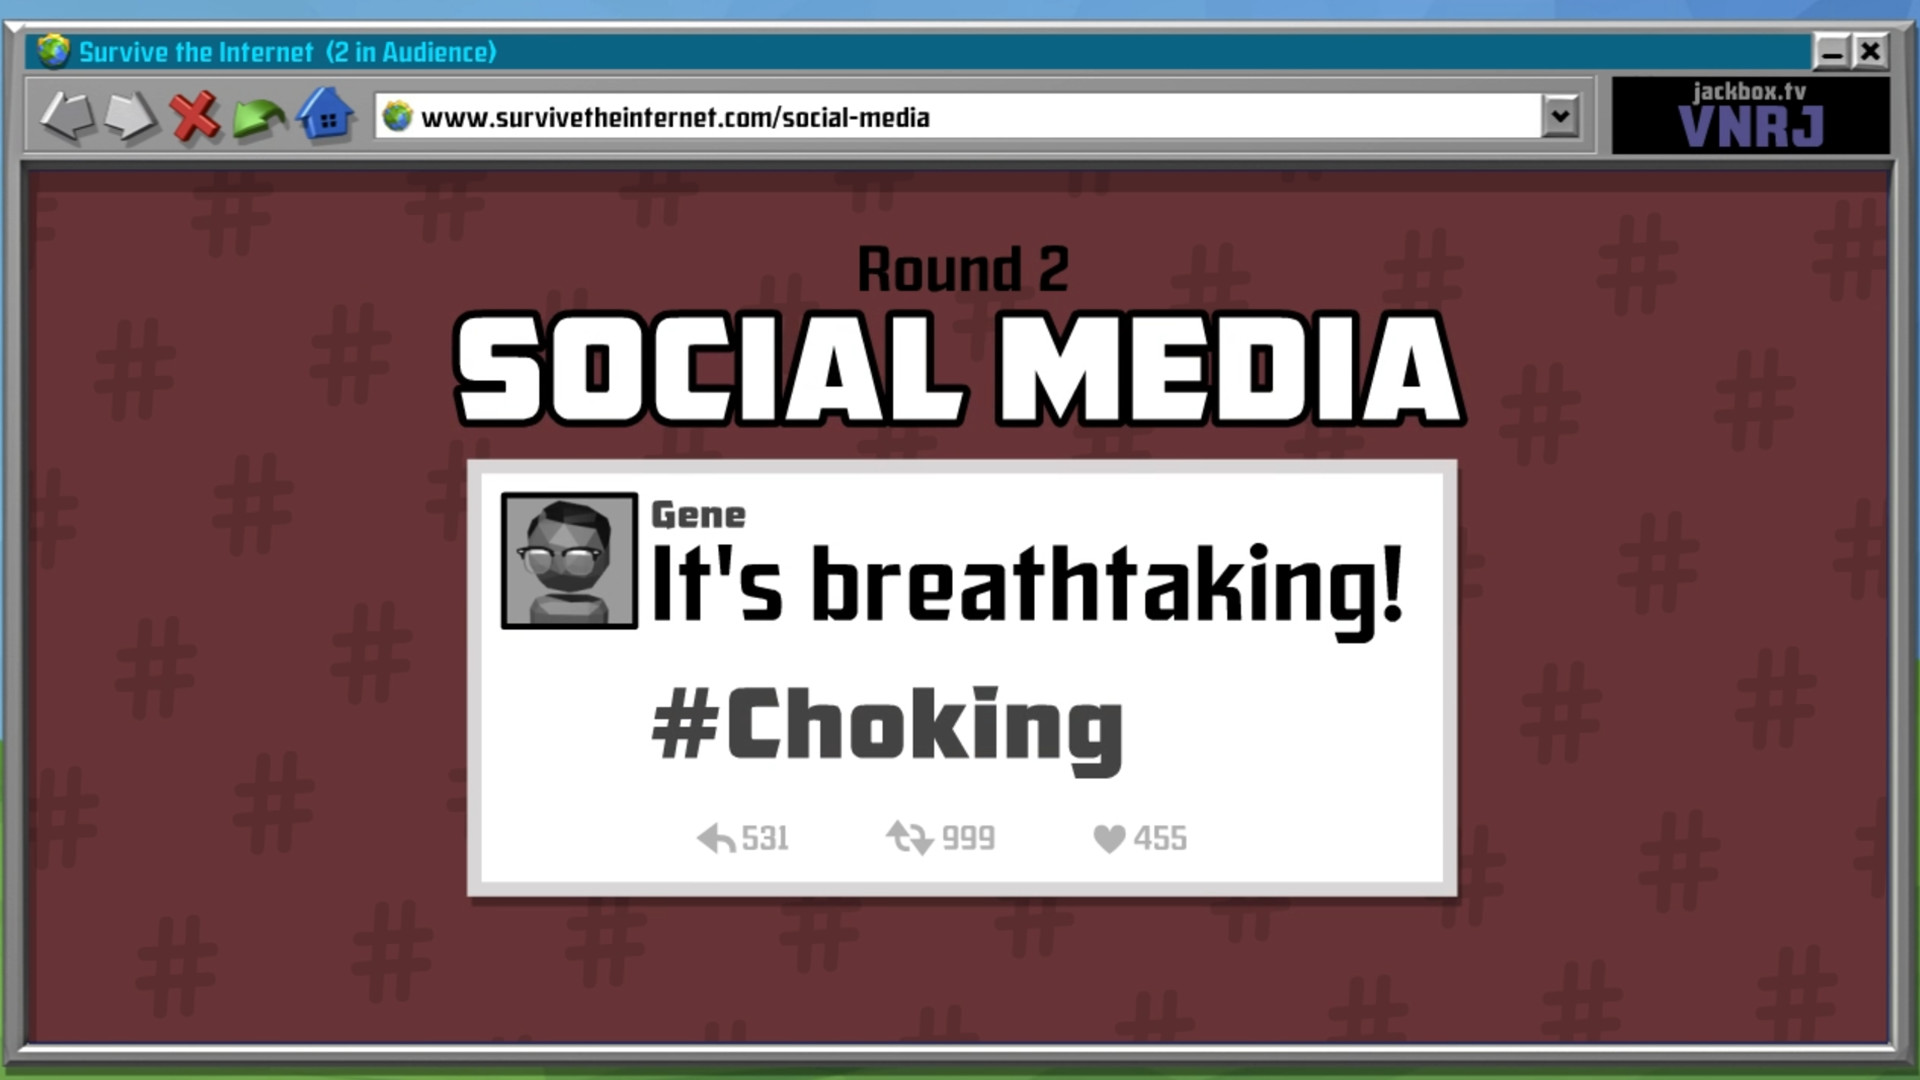
\includegraphics[width=1.0\textwidth]{Cuerpo/4/JPP1.jpg} %
%         \subcaption{Un minijuego de uno de los packs}
%         \label{JPP-Internet}
%     \end{minipage}\hfill
%     \begin{minipage}{0.40\textwidth}
%         \centering
%         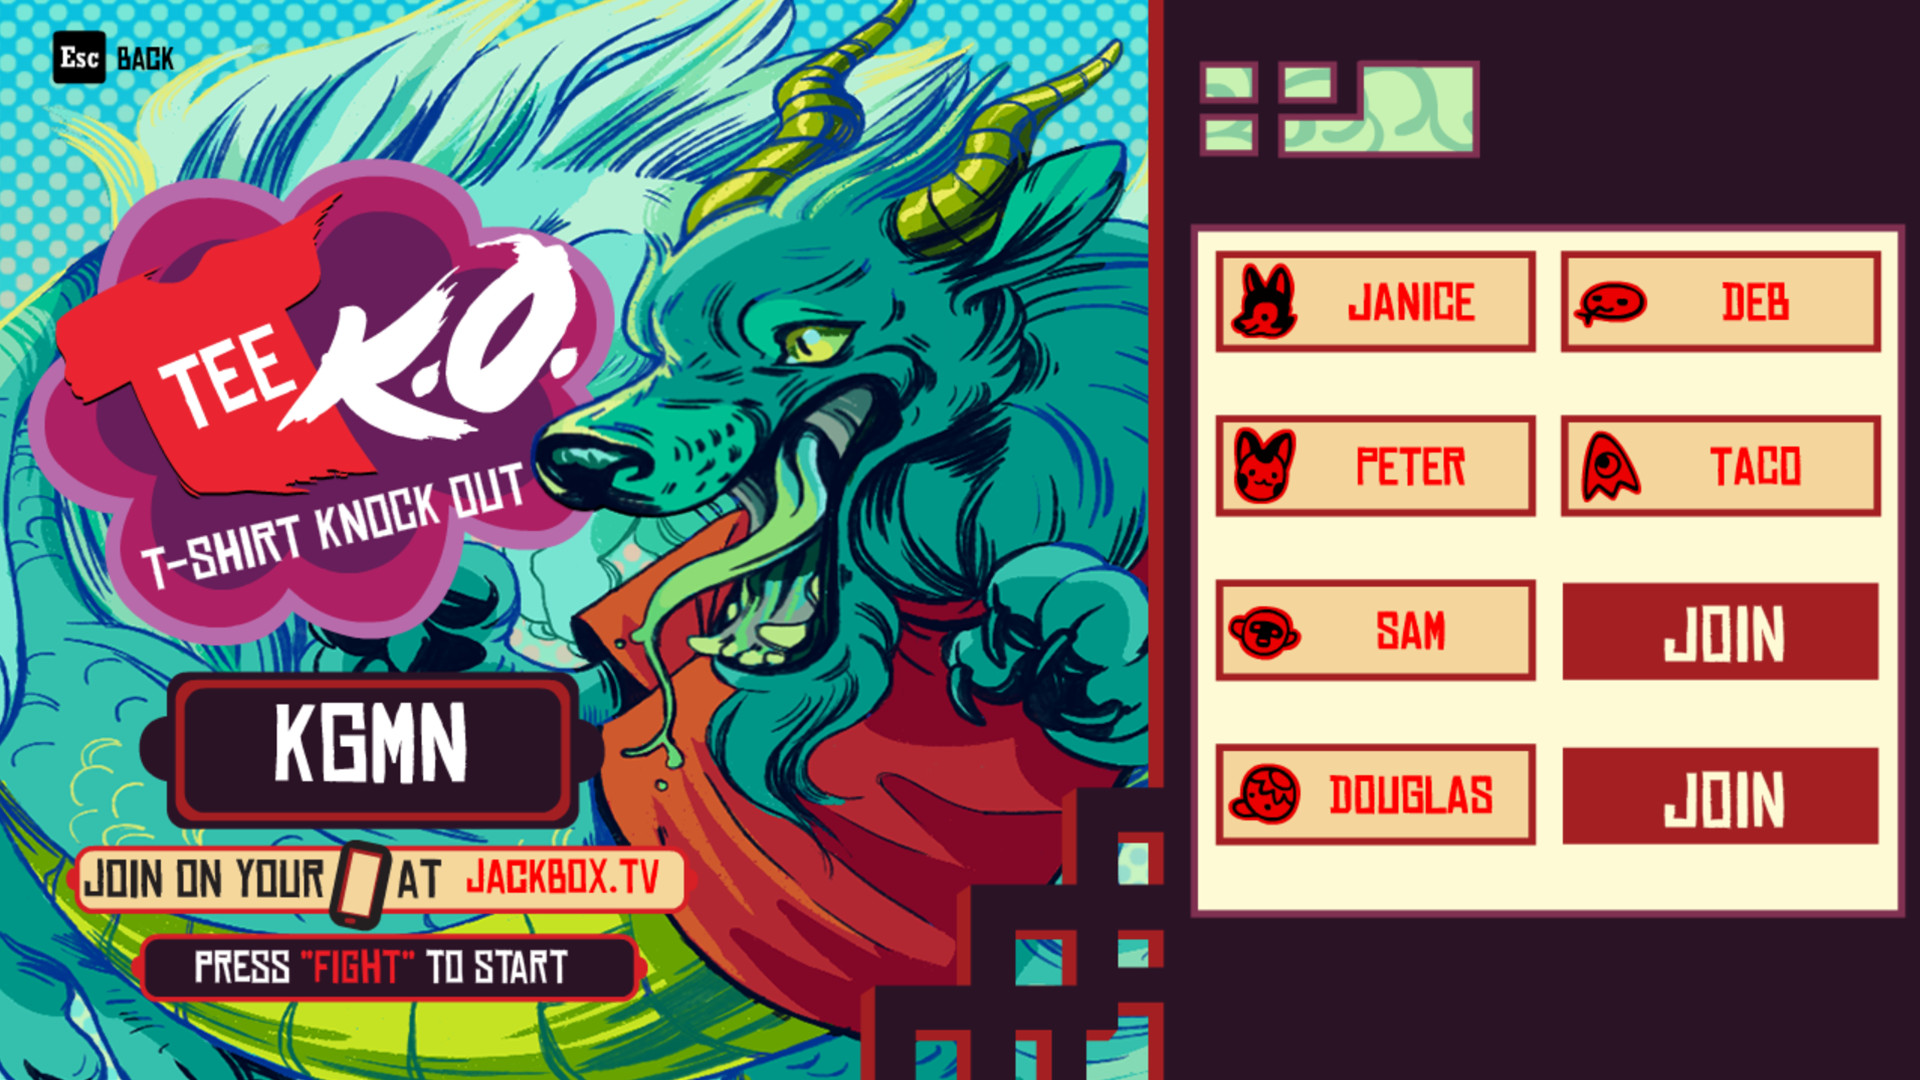
\includegraphics[width=1.0\textwidth]{Cuerpo/4/JPP2.jpg} %
%         \subcaption{Pantalla de inicio de otro minijuego}
%         \label{JPP-Inicio}
%     \end{minipage}
%     \centering
%     \begin{minipage}{0.40\textwidth}
%         \centering
%         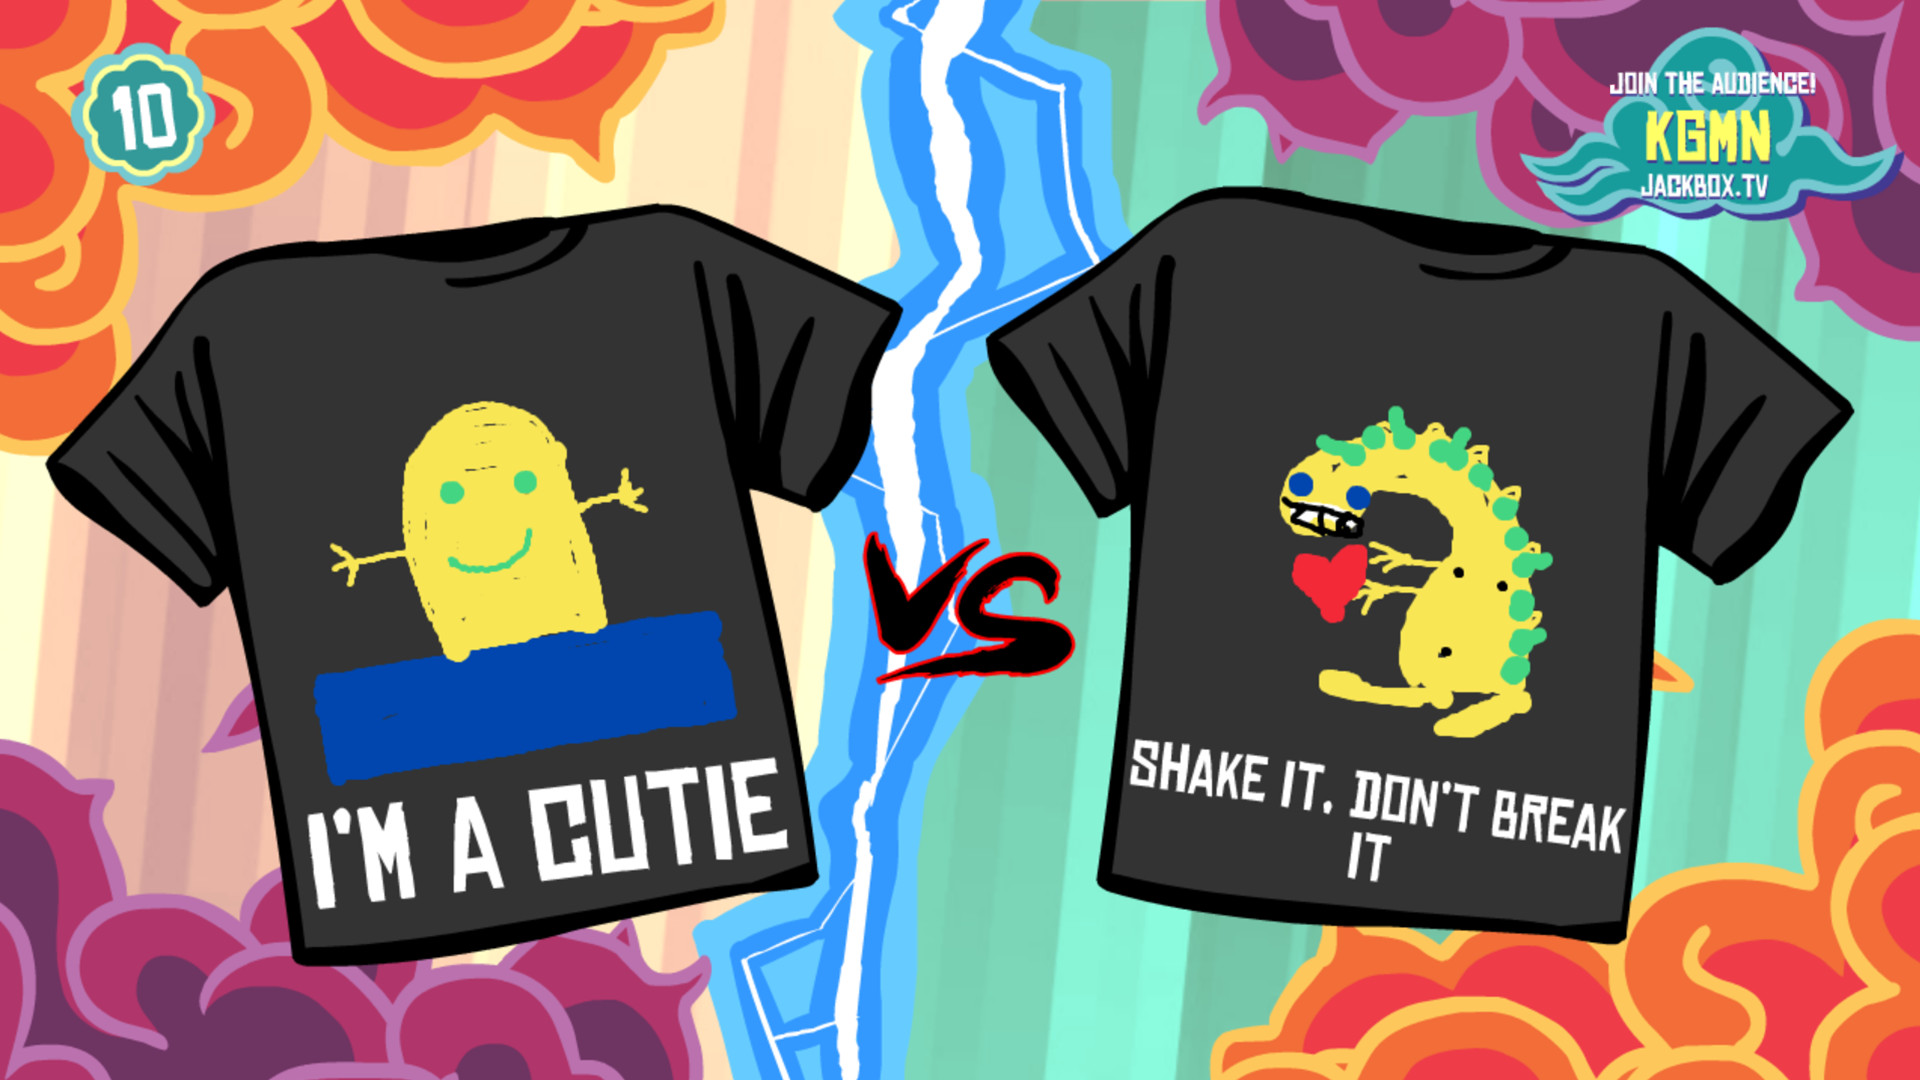
\includegraphics[width=1.0\textwidth]{Cuerpo/4/JPP3.jpg} %
%         \subcaption{Otro minijuego de uno de los packs}
%         \label{JPP-Tees}
%     \end{minipage}
%     \caption{Capturas de varios juegos de los Jackbox Party Packs}
% \end{figure}

% \textbf{Características destacadas:}
% \begin{itemize}
%     \item Tiene una multitud de minijuegos distintos.
%     \item Se caracteriza por tener una velocidad de juego relativamente rápida y
%     una partidas cortas.
%     \item Sólo una persona debe comprar el juego para que varias personas puedan
%     disfrutar del videojuego.
% \end{itemize}

% \textbf{Limitaciones:}
% \begin{itemize}
%     \item El hecho de que el paquete consista de múltiples minijuegos hace que
%     algunos no sean divertidos. Hay demasiada cantidad y poca calidad en
%     general.
%     \item El juego sólo está disponible en inglés.
%     \item Hay que comprar distintas versiones del juego para poder acceder a
%     distintos minijuegos.
% \end{itemize}

% \subsubsection{Pummel Party}
% % Nombre % Desarrollador + Editor % Año de publicación
% \emph{Pummel Party}, desarrollado y publicado por \emph{Rebuilt Games} en el
% 2018, es un juego festivo multijugador usando en la que se destruye a tus
% compañeros con una variedad de objetos y se compite por puntos en una colección
% de minijuegos distintos.

% La página oficial es: % Página web
% \url{http://www.rebuiltgames.com/}

% \textbf{Capturas:}
% \begin{figure}[H]
%     \centering
%     \begin{minipage}{0.40\textwidth}
%         \centering
%         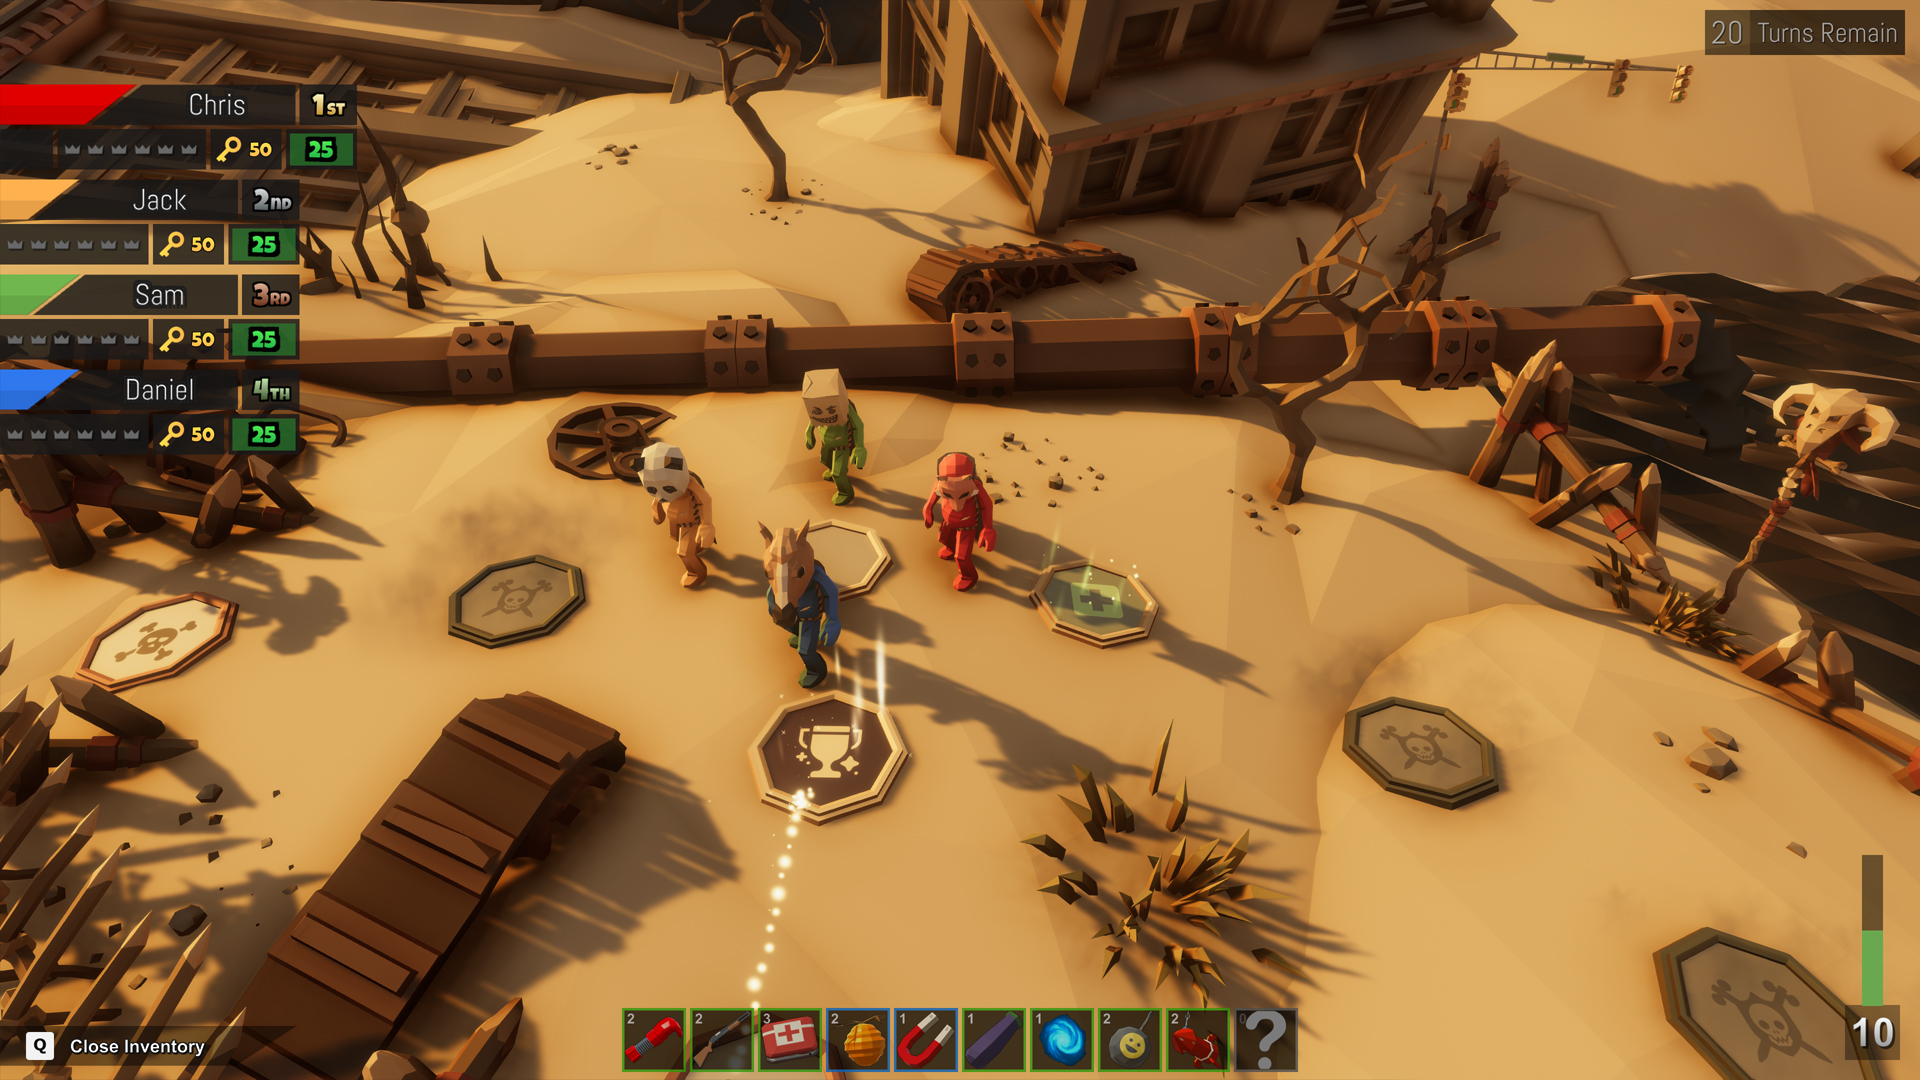
\includegraphics[width=1.0\textwidth]{Cuerpo/4/PMP1.jpg} %
%         \subcaption{El modo tablero de Pummel Party}
%         \label{PMP-Tablero}
%     \end{minipage}\hfill
%     \begin{minipage}{0.40\textwidth}
%         \centering
%         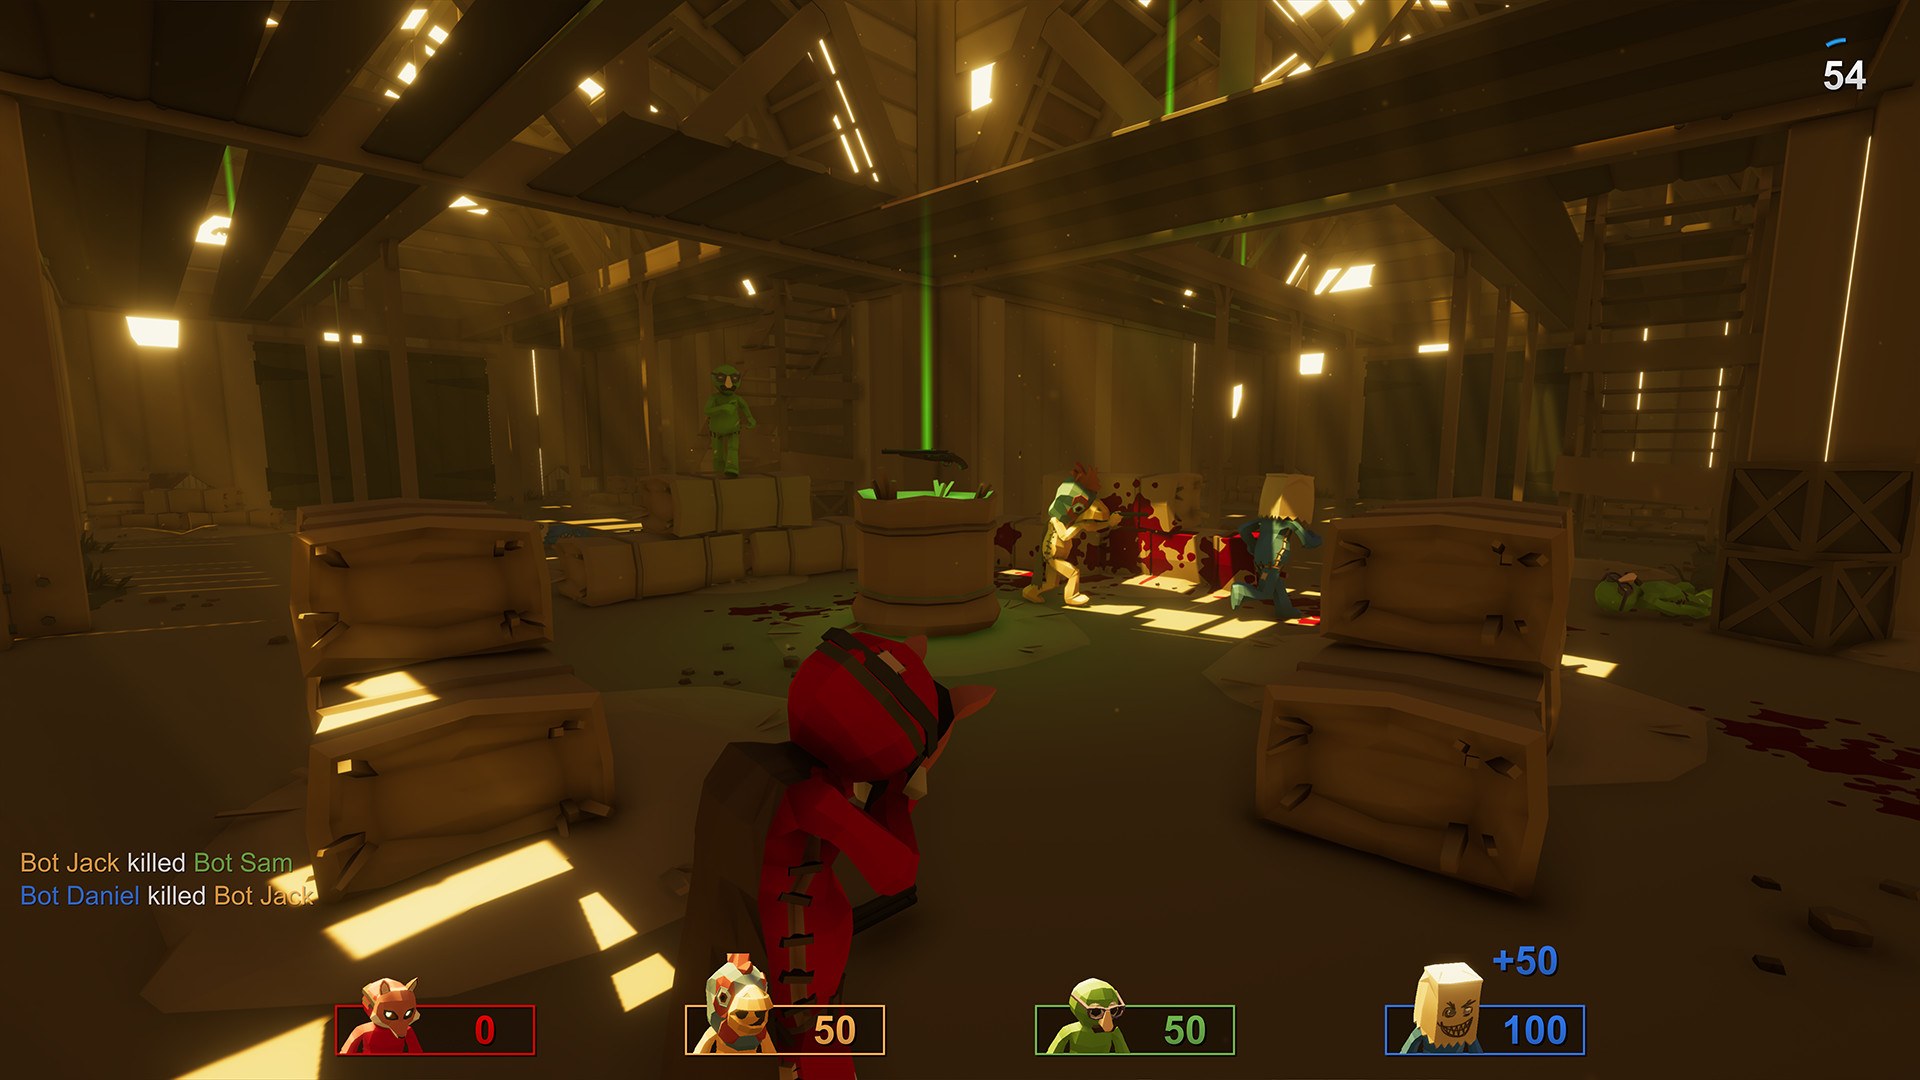
\includegraphics[width=1.0\textwidth]{Cuerpo/4/PMP2.jpg} %
%         \subcaption{Un minijuego de tipo shooter}
%         \label{PMP-Shooter}
%     \end{minipage}
%     \centering
%     \begin{minipage}{0.40\textwidth}
%         \centering
%         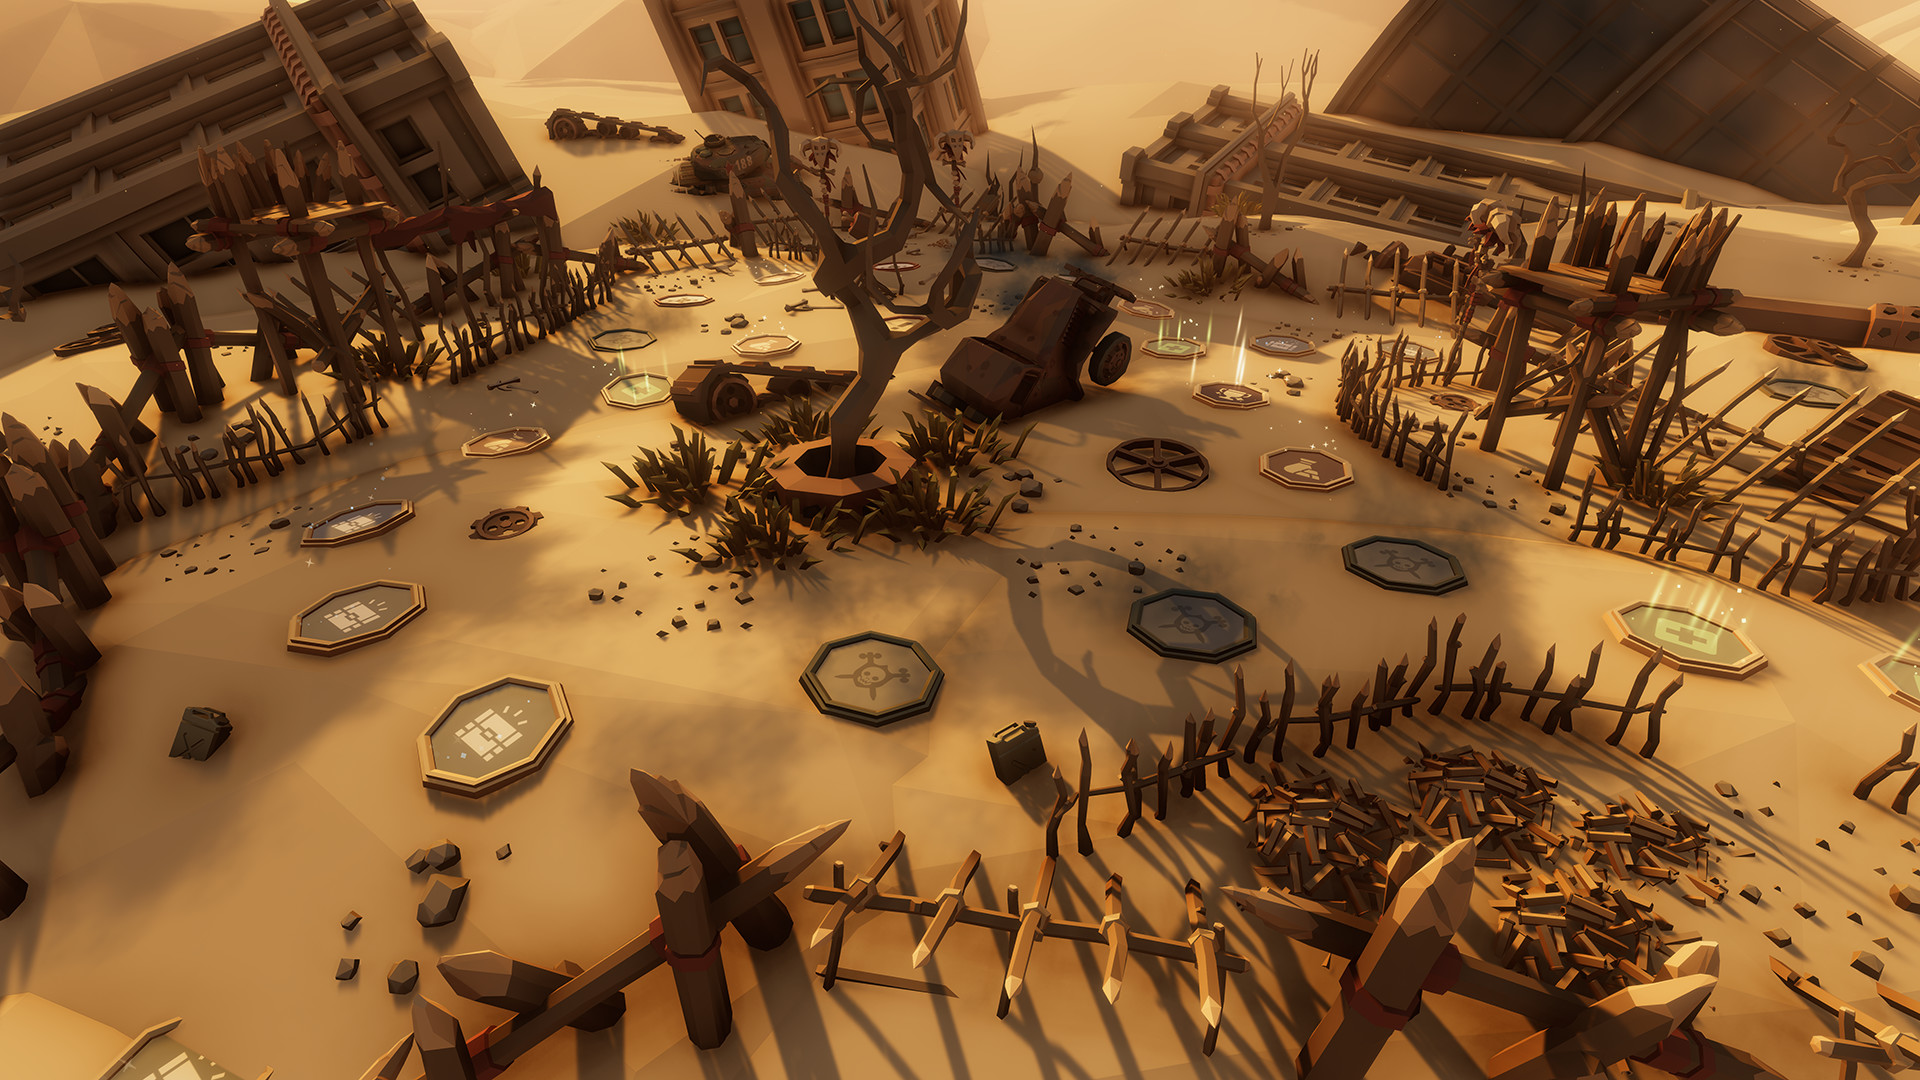
\includegraphics[width=1.0\textwidth]{Cuerpo/4/PMP3.jpg} %
%         \subcaption{Uno de los paisajes de un tablero}
%         \label{PMP-Paisaje}
%     \end{minipage}
%     \caption{Capturas de Pummel Party}
% \end{figure}

% \textbf{Características destacadas:}
% \begin{itemize}
%     \item Una gran cantidad de objetos para destruir a tus amigos.
%     \item Múltiples minijuegos distintos que fomentan la competitividad.
%     \item Traducido a múltiplos idiomas, incluido castellano.
% \end{itemize}

% \textbf{Limitaciones:}
% \begin{itemize}
%     \item El juego es por turnos, por lo cual hay que esperar a que cada jugador
%     tome una acción antes de poder avanzar.
%     \item Sufre de problemas de balance y una AI pobre.
%     \item Puede hacerse demasiado aleatorio y sin sentido a veces.
% \end{itemize}
\section{Comparación de Características} % 3.5 Feature comparison
% \urgent[inline]{Compare your game to the competition. Why would a consumer
% purchase your game over the others?}

\subsection{Ultimate Chicken Horse}

La similitud que tiene el producto con este juego recae en el hecho de que ambos
son de los géneros \emph{festivo} y \emph{plataformas}, se fomenta la
competición entre jugadores y ambos permiten al jugador hacer uso de objetos
especiales para impedir el progreso de los demás competidores.

Sin embargo, podemos observar las siguientes diferencias entre el juego a
desarrollar y \emph{Ultimate Chicken Horse}:
\begin{itemize}
    \item \emph{Ultimate Chicken Horse} permite partidas multijugador local de
    hasta 4 jugadores; mientras que \emph{\izenburua\ } se espera que pueda
    permitir partidas multijugador local de más de 4 personajes.
    \item \emph{Ultimate Chicken Horse} fomenta la competición, pero tiene un
    flujo de juego con cuellos de botella con respecto a la velocidad de
    reacción que se espera de los jugadores. Se espera que \emph{\izenburua\ }
    mantenga un ritmo de juego constamente rápido en todo momento de una
    partida.
    \item \emph{Ultimate Chicken Horse} tiene una lista de niveles cuyos
    entornos individuales se mantienen siempre iguales internamente. Se espera
    que \emph{\izenburua\ } implemente generación procedural para dar más
    variabilidad a los niveles de juego.
    \item Los personajes seleccionables en \emph{Ultimate Chicken Horse} no
    tienen diferencias a nivel de mecánicas de juego o habilidades; mientras que
    se espera que los personajes de \emph{\izenburua\ } sí las tengan.
    \item Las partidas de \emph{Ultimate Chicken Horse} pueden hacerse largas
    debido a los cuellos de botella mencionados anteriormente; mientras que se
    espera que las partidas de \emph{\izenburua\ } sean rápidas y ágiles.
\end{itemize}


\subsection{Jackbox Party Packs}

La similitud que tiene el producto con estos juegos recae en el hecho de que son
todos del género \emph{festivo}, se fomenta la competición entre jugadores y las
partidas suelen ser cortas y rápidas.

Sin embargo, podemos observar las siguientes diferencias entre el juego a
desarrollar y los \emph{Jackbox Party Packs}:
\begin{itemize}
    \item Es necesario comprar distintos juegos/paquetes de \emph{Jackbox Party
    Pack} para ampliar el repertorio de juegos que se pueden experimentar;
    mientras que la compra de \emph{\izenburua\ } será única y contendrá todo el
    contenido en su totalidad.
    \item En los \emph{Jackbox Party Packs} los juegos tienen una fase de
    votación para decidir quién es el ganador; mientras que en \emph{\izenburua\
    } el ganador se decide puramente en base a la habilidad del jugador.
    \item En los \emph{Jackbox Party Packs} no se dispone de objetos especiales
    para progresar o ralentizar el progeso ajeno; mientras que en
    \emph{\izenburua\ } estos serán parte fundamental de cada partida.
    \item Los \emph{Jackbox Party Packs} sólo están disponibles en inglés y han
    sido desarrollados para un público anglosajón, lo cual excluye a gran parte
    del público objetivo de \emph{\izenburua\ }.
    \item Las partidas de \emph{Jackbox Party Packs} son siempre por turnos, lo
    cual hace que la velocidad de reacción no deba ser muy rápida; mientras que
    en \emph{Jackbox Party Packs} se espera una velocidad de reacción rápida en
    todas las partidas.
    \item Muchos minijuegos de los \emph{Jackbox Party Packs} suelen ser
    aburridos para un público cuyo origen cultural no es anglosajón y suele
    haber más cantidad que calidad; mientras que en \emph{\izenburua\ }
    contendrá un humor menos acoplado al origen cultural del público objetivo y
    contendrá modos de juego mejor preparados.
\end{itemize}

\subsection{Pummel Party}

La similitud que tiene el producto con estos juegos recae en el hecho de que
ambos son del género \emph{festivo}, se fomenta la competición entre jugadores y
se hace uso de distintos objetos para progresar en cada partida.

Sin embargo, podemos observar las siguientes diferencias entre el juego a
desarrollar y \emph{Pummel Party}:

\begin{itemize}
    \item En \emph{Pummel Party}, algunos videojuegos sí que contienen elementos
    de acción, pero el modo principal de juego es por turnos, lo cual genera un
    cuello de botella para la velocidad de reacción que se espera del jugador.
    En \emph{\izenburua\ } se espera una velocidad de juego constamente rápida
    cada partida.

    \item Los personajes seleccionables en \emph{Pummel Party} no
    tienen diferencias a nivel de mecánicas de juego o habilidades; mientras que
    se espera que los personajes de \emph{\izenburua\ } sí las tengan.

    \item \emph{Pummel Party} puede llegar a sufrir problemas de balance en
    muchas partidas. Se espera que los elementos y objetos de \emph{\izenburua\
    } sean adecuadamente balanceados.
\end{itemize}

\section{Sales expectations} % 3.6 Sales expectations
\urgent{Provide an estimate of sales over the first year broken down by quarter.
How many units will be sold globally, as well as within key markets, like the
United States, England, Japan, etc.?}

% \chapter{Estudio de Mercado}

3 videojuegos similares

    1. Título
    2. Compañía
    3. Plataformas
    4. Modelo de negocio
    5. Web oficial
    6. Captura de pantalla
    7. Aspectos positivos
    8. Aspectos negativos

Primer videojuego:
    MicroMages
    MorphCat Games
    PC y NES
    Buy-to-Play (https://en.wikipedia.org/wiki/Buy-to-play)
    https://morphcatgames.itch.io/micromages
    https://www.youtube.com/watch?v=VFX401vvKTQ
    (Captura aquí)
    (Aspectos positivos)
    (Aspectos negativo)

Segundo videojuego (quizás Kirby no, igual Ultimate Chicken Horse):
    Kirby Crytal Shards (Minigames)
    Nintendo + HAL Laboratory
    Nintendo 64
    Buy-to-Play
    https://kirby.nintendo.com/ (\url{https://en.wikipedia.org/wiki/Kirby_64\%3A_The_Crystal_Shards})
    (Captura aquí)
    (Aspectos positivos)
    (Aspectos negativos)

Tercer videojuego:
    Risk of Rain
    Hopo Games + Gearbox Publishing
    PC + others
    Buy-to-Play
    https://www.riskofrain.com/
    https://riskofraingame.com/
    \url{https://store.steampowered.com/app/248820/Risk_of_Rain/}
    (Captura aquí)
    (Aspectos positivos)
    (Aspectos negativos)

\section{Género}

Platformer and Party Game

\section{Audiencia}

\subsection{Segmento demográfico}
People that want fast play

\subsection{Plan de comercialización}
Sold through Steam (Buy-to-Play)

\section{Competidores}

% Human Fall Flat

Super Meat Boy

Celeste

Fall Guys
    * Características destacadas:
    * Limitaciones:

Pummel Party
    * Características destacadas:
    * Limitaciones:

Stick Fight: The Game
    * Características destacadas:
    * Limitaciones:

Ultimate Chicken Horse
    * Características destacadas:
    * Limitaciones:

Jackbox Party Packs
    * Características destacadas:
    * Limitaciones:

\subsection{Características destacadas}

\subsection{Limitaciones}
 % NO

\chapter{Modelo de Negocio}

Pay-to-play
Suscripción
Free-to-play
Pay-to-win
Freemium
Shareware

\chapter{Personajes de juego}

\section{Character design} % 6.1 Character design
This is where you describe any game characters and their attributes.
\section{Types} % 6.2 Types

\subsection{PCs (Player Characters)} % 6.2.1 PCs (player characters)

\begin{itemize} % Nombres que tengan que ver con marionetas, actores y actrices manipulad@s
    \item Jim
    \item Truman
    \item ...
\end{itemize}

\subsection{NPCs (Non-Player Characters)} % 6.2.2 NPCs (nonplayer characters):

If your game involves character types, you will need to treat each one as an
object, defining its properties and functionality.

\begin{itemize}
    \item Oxymandias (The Host, The Lich King)
    \item The monsters/Enemies (?)
    \item Bosses
    \item Vendors
    \item The eyes/Cameras (Are these objects?)
\end{itemize}

\subsubsection{Behaviour} % 6.2.2.1 Behavior

\subsubsection{AI} % 6.2.2.2 AI

% \chapter{Otros elementos de juego}

\section{Tipos} % 6.2 Types

% \change[inline]{If your game involves character types, you will need to treat
% each one as an object, defining its properties and functionality.}

\subsection{Objetos mágicos}

\subsection{Objetos recursos}

\subsection{Plataformas}

\subsection{Trampas}
\section{Descripción de elementos} % 6.1 Character design

% \change[inline]{This is where you describe any game characters and their
% attributes.}


% \chapter{Story}
\section{Synopsis} % 7.1 Synopsis
If your game includes a story, summarize it here. Keep it down to one or two paragraphs.

\section{Complete story}% 7.2 Complete story
This is your chance to outline the entire story. Do so in a way that mirrors the gameplay. Do not just tell your story, but structure it so that it unfolds as the game progresses.

\subsection{Backstory}% 7.3 Backstory
Describe any important elements of your story that do not tie directly into the gameplay. Much of this might not actually make it into the game, but it might be good to have it for reference.

\subsection{Narrative devices}% 7.4 Narrative devices
Describe the various ways in which you plan to reveal the story. What are the devices you plan to use to tell the story?

\subsection{Subplots}% 7.5 Subplots
Because games are not linear like books and movies, there might be numerous smaller stories interwoven into the main story. Describe each of these subplots and explain how they tie into the game-play and the master plot.

\subsubsection{Subplot 1}%     7.5.1 Subplot #1
¿Qué pasa aquí?
\subsubsection{Subplot 2}%     7.5.2 Subplot #2
¿Qué pasa aquí? % NO para esta entrega
% \chapter{El mundo del juego}

\change[inline]{If your game involves the creation of a world, you may want to
go into detail on all aspects of that world.}

\section{Resumen} % 8.1 Overview
Resumen del juego
\section{Sitios importantes} % 8.2 Key locations
Sitios importantes
\section{Travel} % 8.3 Travel
¿Cómo se viaja?
\section{Mapping} % 8.4 Mapping
Mapa (?)
\section{Scale} % 8.5 Scale
Escala (?)
\section{Physical objects} % 8.6 Physical objects
\section{Condiciones climáticas} % 8.7 Weather conditions
\section{Day and night} % 8.8 Day and night
\section{Tiempo} % 8.9 Time
\section{Physics} % 8.10 Physics
\section{Sociedad/cultura} % 8.11 Society/culture % NO para esta entrega
% \chapter{Media List}
List all of the media that will need to be produced. The specifics of your game
will dictate what categories you need to include. Be detailed with this list,
and create a file naming convention up front. This can avoid a lot of confusion
later on.

\section{Interface assets} % 9.1 Interface assets
\section{Environments} % 9.2 Environments


\section{Characters} % 9.3 Characters


\section{Animation} % 9.4 Animation
\section{Music and sound effects} % 9.5 Music and sound effects
 % NO
% \chapter{Technical Spec}
As mentioned, the technical spec is not always included in the design document. Often it is a separate document prepared in conjunction with the design document. This spec is prepared by the technical lead on the project.

\section{Technical analysis} % 10.1 Technical analysis
\subsection{New technology} % 10.1.1 New technology
Is there any new technology that you plan on developing for this game? If so, describe it in detail.

\subsection{Major software development tasks} % 10.1.2 Major software development tasks
Do you need to do a lot of software development for the game to work? Or are you simply going to license someone else's engine or use a preexisting engine that you have created?

\subsection{Risks} % 10.1.3 Risks
What are the risks inherent in your strategy?

\subsection{Alternatives} % 10.1.4 Alternatives
Are there any alternatives that can lower the risks and the cost?

\subsection{Estimated resources required} % 10.1.5 Estimated resources required
Describe the resources you would need to develop the new technology and software needed for the game.
\section{Development platform and tools Describe the development} % 10.2 Development platform and tools
Describe the development platform, as well as any software tools and hardware that are required to produce the game.
\subsection{Software} % 10.2.1 Software

\subsection{Hardware} % 10.2.2 Hardware
\section{Delivery} % 10.3 Delivery
How do you plan to deliver this game? Over the Internet? Via an app service? At a brick-and-mortar location? What is required to accomplish this?
\subsection{Required hardware and software} % 10.3.1 Required hardware and software

\subsection{Required materials} % 10.3.2 Required materials
\section{Game engine} % 10.4 Game engine
\subsection{Technical specs} % 10.4.1 Technical specs
What are the specs of your game engine?

\subsection{Design} % 10.4.2 Design
Describe the design of your game engine.
\subsubsection{Features} % 10.4.2.1 Features

\subsubsection{Details} % 10.4.2.2 Details

\subsection{Collision detection} % 10.4.3 Collision detection
If your game involves collision detection, how does it work?
\subsubsection{Features} % 10.4.3.1 Features

\subsubsection{Details} % 10.4.3.2 Details
\section{Interface technical specs} % 10.5 Interface technical specs
This is where you describe how your interface is designed from a technical perspective. What tools do you plan to use, and how will it function?
\subsection{Features} % 10.5.1 Features

\subsection{Details} % 10.5.2 Details
\section{Controls and technical specs} % 10.6 Controls & technical specs
This is where you describe how your controls work from a technical perspective. Are you planning on supporting any unusual input devices that would require specialized programming?
\subsection{Features} % 10.6.1 Features

\subsection{Details} % 10.6.2 Details
\section{Lighting models} % 10.7 Lighting models
Lighting can be a substantial part of a game. Describe how it works and the features that you require.
\subsection{Modes} % 10.7.1 Modes
\subsubsection{Features} % 10.7.1.1 Features

\subsubsection{Details} % 10.7.1.2 Details

\subsection{Models} % 10.7.2 Models
\subsection{Light sources} % 10.7.3 Light sources
\section{Rendering system} % 10.8 Rendering system
\subsection{Technical specs} % 10.8.1 Technical specs

\subsection{2D/3D rendering} % 10.8.2 2D/3D rendering

\subsection{Camera} % 10.8.3 Camera
\subsubsection{Operation} % 10.8.3.1 Operation

\subsubsection{Features} % 10.8.3.2 Features

\subsubsection{Details} % 10.8.3.3 Details
\section{Internet/network spec} % 10.9 Internet/network spec
If your game requires an Internet connection, you should make that clear in the specs.
\section{System parameters} % 10.10 System parameters
I won't go into detail on all the possible system parameters, but suffice to say that the design document should list them all and describe their functionality.
\subsection{Max players} % 10.10.1 Max players

\subsection{Servers} % 10.10.2 Servers

\subsection{Customization} % 10.10.3 Customization

\subsection{Connectivity} % 10.10.4 Connectivity

\subsection{Websites} % 10.10.5 Websites

\subsection{Persistence} % 10.10.6 Persistence

\subsection{Saving games} % 10.10.7 Saving games

\subsection{Loading games} % 10.10.8 Loading games

\section{Other} % 10.11 Other
This section is for any other technical specifications that should be included, such as help menus, manuals, setup and installation routines, etc.
\subsection{Help} % 10.11.1 Help

\subsection{Manual} % 10.11.2 Manual

\subsection{Setup} % 10.11.3 Setup
 % NO

\cleardoublepage
% \chapter{Conclusión}
\lipsum[12]

\cleardoublepage
}

%------------ Elementos finales ------------%
{
\backmatter % La zona de índices, bibliografía y referencias
\pagestyle{plain}
% % \fancyhead[LE,RO]{\small\slshape\thepage}
% \fancyhead[LO,RE]{\small\slshape \nouppercase{\leftmark}}

\printbibliography[heading=bibintoc,title={Bibliografía}] %Prints the entire bibliography with the title "Bibliografía"

% \clearpage

%Filters bibliography
% \printbibliography[heading=subbibintoc,type=article,title={Articles only}]
% \printbibliography[type=book,title={Books only}]

% \printbibliography[keyword={physics},title={Physics-related only}]
% \printbibliography[keyword={latex},title={\LaTeX-related only}]
\cleardoublepage
}

%------------ Anexos del informe ------------%
{
% \noappendicestocpagenum
% \appendixpage
% \addappheadtotoc
% \appendix % La zona de apéndices
% % reinstate the correct level for list of tables and figures
% \appto\appendix{\addtocontents{toc}{\protect\setcounter{tocdepth}{0}}}
% \appto\listoffigures{\addtocontents{lof}{\protect\setcounter{tocdepth}{1}}}
% \appto\listoftables{\addtocontents{lot}{\protect\setcounter{tocdepth}{1}}}
% \pagestyle{fancy-end}
% \chapter{Artefactos relacionados a la planificación del proyecto}
\section{Esquema de Descomposición de Trabajo}

\begin{figure}[H]
    \centering
    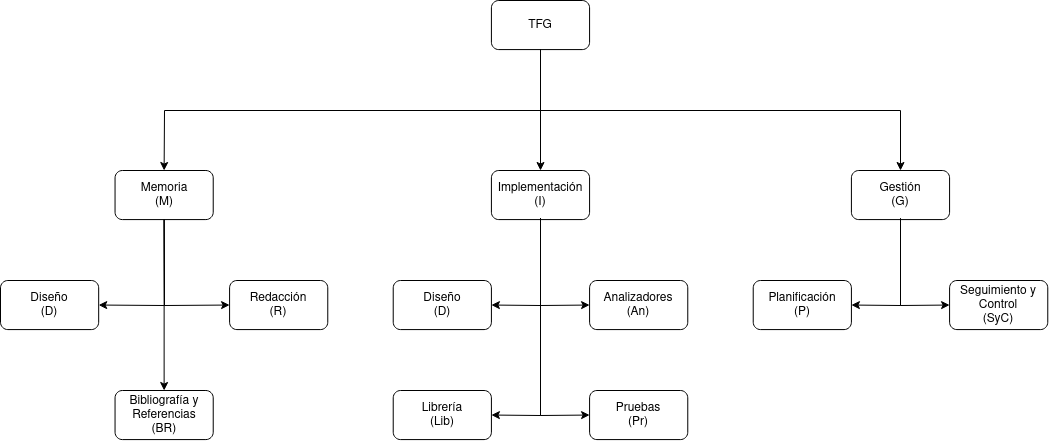
\includegraphics[width=\textwidth]{8-Apéndices/EDT.png}
    \caption{Esquema de Descomposición de Trabajo del Proyecto}
    \label{fig:EDT}
\end{figure}

\cleardoublepage
}

\end{document}